\documentclass[main.tex]{subfiles}
\begin{document}
\begin{enumerate}

\item[1.] Given the following training data set in the format: \textit{input $\rightarrow$ label}
\begin{itemize}[label={}]
    \item $[23,23,23] \rightarrow 358$
    \item $[15,15,15] \rightarrow 230$
    \item $[10,13,15] \rightarrow 211$
    \item $[7,17,27] \rightarrow 302$
\end{itemize}
Consider forward propagation, initialize the weighting vector $[1,2,3]$, bias $b=20$, and use $y=\vec{w}^{T}\vec{x}+b$ to calculate the output/prediction.
    \begin{enumerate}
        \item Calculate the mean square error (MSE) (i.e. cost function for linear regression) for the training set. Use backpropagation to reduce the MSE by updating the weights matrix and bias.
        
        \begin{itemize}[label={}]
            \item $\hat{y}_1 = \left(1*23+2*23+3*23\right)+20= 158$
            \item ${y}_1 = 358$
            \item $\hat{y}_2 = \left(1*15+2*15+3*15\right)+20= 110$
            \item ${y}_2 = 230$
            \item $\hat{y}_3 = \left(10*1+13*2+15*3\right)+20= 101$
            \item ${y}_3 = 211$
            \item $\hat{y}_4 = \left(7*1+17*2+27*3\right)+20= 142$
            \item ${y}_4 = 302$
            \item $\text{MSE} = E(X,\theta) = \frac{1}{2N}\sum_{i=1}^{N}\left(y_i-\hat{y_i}\right)^2$
            \item $E(X,\theta) = \frac{1}{8}\left(\left (358-158\right)^2+\left(230-110\right)^2+\left(211-101\right)^2+\left(302-142\right)^2\right)$
            \item $E(X,\theta) = 11512.5$
        \end{itemize}
        
        \item Calculate the partial derivatives $\frac{\partial \text { cost }}{\partial \text{weight}}, \frac{\partial \text { cost }}{\partial \text { output }}, \frac{\partial \text { cost }}{\partial \text { bias }}$ for the first row of the data. Calculate the cost (squared error) for the first row of the data . The partial derivative of $\frac{\partial \text { cost }}{\partial \text { weight }}$ has the form $[a_1,a_2,a_3]$. \\

        Definitions
        
        \begin{itemize}[label={}]
            \item $w_{ij}^k$: weight for node $j$ in layer $l_k$ for incoming node $i$
            \item $b_{i}^{k}$: bias for node i in layer $l_k$
            \item $a_{i}^{k}$: product sum plus bias (activation) for node $i$ in layer $l_k$
            \item $o_{i}^{k}$: output for node $i$ in layer $l_k$
            \item $r_k$: number of nodes in layer $l_k$
            \item $g$: activation function for the hidden layer nodes
            \item $g_0$: activation function for the output layer nodes
        \end{itemize}
        
        The error function in classic backpropagation is the mean squared error 
        
        \begin{equation} \label{meanSquaredError}
        E(X, \theta)=\frac{1}{2 N} \sum_{i=1}^{N}\left(\hat{y}_{i}-y_{i}\right)^{2}
        \end{equation}
        
        where $y_i$ is the target value for input-output pair $\left(\vec{x}_{i}, y_{i}\right)$ and $\hat{y_i}$ is the computed output of the network on input $\vec{x}_i$. For the first row of data the squared error is $\left(\hat{y}_{1}-y_{1}\right)^{2}=\left (358-158\right)^2=40000$. To simplify the mathematics, the bias $b_i^k$ for node $i$ in layer $k$ will be incorporated into the weights as $w_{0i}$, with a fixed output of $o_0^{k-1} = 1$ for node $0$ in the layer $k-1$. Thus $w_{0i}^k = b_i^k$, and 
        
        \begin{equation} \label{productSumBias}
        a_{i}^{k}=b_{i}^{k}+\sum_{j=1}^{r_{k-1}} w_{j i}^{k} o_{j}^{k-1}=\sum_{j=0}^{r_{k-1}} w_{j i}^{k} o_{j}^{k-1}
        \end{equation}
        
        where the left side is the original formulation and the right side is the new formulation. Backpropagation attempts to minimize the error function with respect to the neural networks weights by calculating, for each weight $w_{ij}^{k}$, the value of $\frac{\partial E}{\partial w_{i j}^{k}} = \frac{\partial \text { cost }}{\partial \text{weight}}$. The error function can be decomposed into a sum over individual error terms for each individual input-output pair, and the derivative can be calculated with respect to each  input-output pair individually and then combined.
        
        \begin{equation} \label{partialErrorPartialWeightDecomposedSum}
        \frac{\partial E(X, \theta)}{\partial w_{i j}^{k}}=\frac{1}{N} \sum_{d=1}^{N} \frac{\partial}{\partial w_{i j}^{k}}\left(\frac{1}{2}\left(\hat{y}_{d}-y_{d}\right)^{2}\right)=\frac{1}{N} \sum_{d=1}^{N} \frac{\partial E_{d}}{\partial w_{i j}^{k}}
        \end{equation}
        
        For the purposes of derivation, the backpropagation algorithm concerns itself with only one input-output pair. Once this is derived, the general form for all input-output pairs in $X$ can be generated by combining the individual gradients, with the error function for derivation 
        
        \begin{equation} \label{errorFunction}
        E=\frac{1}{2}(\hat{y}-y)^{2}
        \end{equation}
        
        where the subscript d in $E_d$, $\hat{y}_d$, and $y_d$ is omitted for simplification. The derivation of the backpropagation algorithm begins by applying the chain rule to the error function partial derivative 
       
        \begin{equation} \label{partialErrorPartialWeightChainRule}
        \frac{\partial E}{\partial w_{i j}^{k}}=\frac{\partial E}{\partial a_{j}^{k}} \frac{\partial a_{j}^{k}}{\partial w_{i j}^{k}}
        \end{equation}
       
        where $a_j^k$ is the activation (product-sum plus bias) of node $j$ in layer $k$ before it is passed to the nonlinear activation function (in this case, the sigmoid function) to generate the output. The first term is referred to as the \textbf{error}
        
        \begin{equation} \label{error}
        \delta_{j}^{k} \equiv \frac{\partial E}{\partial a_{j}^{k}},
        \end{equation}
       
        and the second term can be calculated from the equation for $a_j^k$  
        
        \begin{equation} \label{partialActivationPartialWeight}
        \frac{\partial a_{j}^{k}}{\partial w_{i j}^{k}}=\frac{\partial}{\partial w_{i j}^{k}}\left(\sum_{l=0}^{r_{k-1}} w_{l j}^{k} o_{l}^{k-1}\right)=o_{i}^{k-1}.
        \end{equation}
        
        resulting in the partial derivative of the error function $E$ with respect to a weight $w_{ij}^k$ 
        
        \begin{equation} \label{partialErrorPartialWeightRedefined}
        \frac{\partial E}{\partial w_{i j}^{k}}=\delta_{j}^{k} o_{i}^{k-1}.
        \end{equation}
        
        Thus, the partial derivative of a weight is a product of the error term $\delta_j^k$ at node $j$ in layer $k$, and the output $o_i^{k-1}$ of node $i$ in layer $k-1$. This makes intuitive sense since the weight $w_{ij}^{k}$ connects the output of node $i$ in layer $k-1$ to the input of node $j$ in layer $k$ in the computation graph. Starting from the final layer, backpropagation attempts to define the value $\delta_{1}^{m}$, where $m$ is the final layer (the subscript is 1 and not j because this derivation concerns a one-output neural network, so there is only one output node $j=1$). Expressing the error function $E$ in terms of the value $a_1^m$ (since $\delta_1^m$ is a partial derivative with respect to $a_1^m$) gives 
        
        \begin{equation} \label{errorFunctionInTermsOfActivation}
        E=\frac{1}{2}(\hat{y}-y)^{2}=\frac{1}{2}\left(g_{o}\left(a_{1}^{m}\right)-y\right)^{2},
        \end{equation}
        
        where $g_{o}(x)$ is the activation function of the output layer. Apply the partial derivative and use the chain rule 
        
        \begin{equation} \label{errorNodeOneFinalLayer}
        \delta_{1}^{m}=\left(g_{0}\left(a_{1}^{m}\right)-y\right) g_{o}^{\prime}\left(a_{1}^{m}\right)=(\hat{y}-y) g_{o}^{\prime}\left(a_{1}^{m}\right)
        \end{equation}
        
        and the partial derivative of the error function $E$ with respect to a weight in the final layer $w_{i1}^m$ is 
        
        \begin{equation} \label{partialErrorPartialWeightFinalLayer}
        \frac{\partial E}{\partial w_{i 1}^{m}}=\delta_{1}^{m} o_{i}^{m-1}=(\hat{y}-y) g_{o}^{\prime}\left(a_{1}^{m}\right) o_{i}^{m-1}.
        \end{equation}
    
        For error term $\delta_j^k$ in layer $1 \leq k<m$
        
        \begin{equation} \label{errorLayerK}
        \delta_{j}^{k}=\frac{\partial E}{\partial a_{j}^{k}}=\sum_{l=1}^{r^{k+1}} \frac{\partial E}{\partial a_{l}^{k+1}} \frac{\partial a_{l}^{k+1}}{\partial a_{j}^{k}},
        \end{equation}
        
        where $l$ ranges from 1 to $r^{k+1}$ (the number of nodes in the next layer). Since the bias input $o_0^k$ corresponding to $w_{0j}^{k+1}$ is fixed, its value is not dependent on the outputs of previous layers, and thus $l$ does not take on the value $0$. Adding the error term $\delta_l^{k+1}$
        
        \begin{equation} \label{errorLayerKErrorLayerK+1}
        \delta_{j}^{k}=\sum_{l=1}^{r^{k+1}} \delta_{l}^{k+1} \frac{\partial a_{l}^{k+1}}{\partial a_{j}^{k}},
        \end{equation}
        
        and the definition of $a_l^{k+1}$
        
        \begin{equation} \label{activationLKPlusOne}
        a_{l}^{k+1}=\sum_{j=1}^{r^{k}} w_{j l}^{k+1} g\left(a_{j}^{k}\right),
        \end{equation}
        
        where $g(x)$ is the activation function for the hidden layers,
        
        \begin{equation} \label{partialActivationLK+1PartialActivationJK}
        \frac{\partial a_{l}^{k+1}}{\partial a_{j}^{k}}=w_{j l}^{k+1} g^{\prime}\left(a_{j}^{k}\right).
        \end{equation}
        
        Inserting equation \ref{partialActivationLK+1PartialActivationJK} into equation \ref{errorLayerKErrorLayerK+1} yields equation \ref{backpropagationFormula}, referred to as the backpropagation formula, for the error term $\delta_j^k$ in the hiden layers.
        
        \begin{equation} \label{backpropagationFormula}
        \delta_{j}^{k}=\sum_{l=1}^{r^{k+1}} \delta_{l}^{k+1} w_{j l}^{k+1} g^{\prime}\left(a_{j}^{k}\right)=g^{\prime}\left(a_{j}^{k}\right) \sum_{l=1}^{r^{k+1}} w_{j l}^{k+1} \delta_{l}^{k+1}
        \end{equation}
        
        Inserting equation \ref{backpropagationFormula} into equation \ref{partialErrorPartialWeightRedefined} yields equation \ref{partialErrorPartialWeightNodesIJLayerK}, the partial derivative of the error function $E$ with respect to a weight in the hidden layers $w_{ij}^{k}$ for $1 \leq k < m$.
    
        \begin{equation}\label{partialErrorPartialWeightNodesIJLayerK}
        \frac{\partial E}{\partial w_{i j}^{k}}=\delta_{j}^{k} o_{i}^{k-1}=g^{\prime}\left(a_{j}^{k}\right) o_{i}^{k-1} \sum_{l=1}^{r^{k+1}} w_{j l}^{k+1} \delta_{l}^{k+1}
        \end{equation}
    
        \item Update the weights with $\frac{\partial \text{cost}}{\partial \text { weight }}, \frac{\partial \text { cost }}{\partial \text { bias }}$ from the fist row of the data using the learning rates $LR_1 = 0.0001$ and $LR_2 = 0.001$. Then recalculate the MSE for both rates. What happens to the learning process for using each rate? Thus, which learning rate is better suited for training, why? 
        
        \begin{figure}
        \centering\fbox{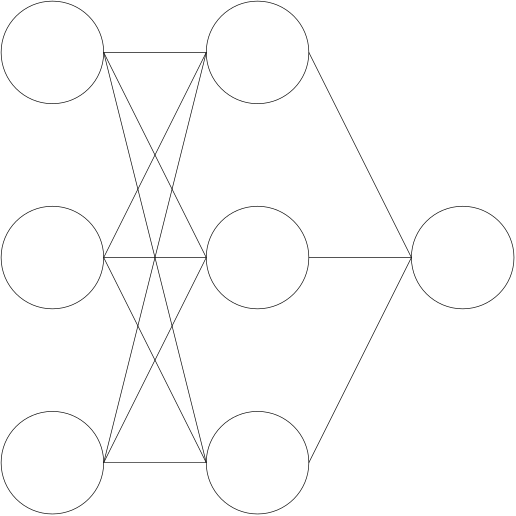
\includegraphics[height=3.0in]{figures/hw3/hw3_1.png}}
        \caption{Feedforward fully connected three input one hidden layer one output neural network. Calculation of the forward phase for each input-output pair $\left(\vec{x}_{d}, y_{d}\right)$ (example $\left(\vec{x}_{1}, y_{1}\right) = [23,23,23] \rightarrow 358$) and the results $\hat{y}_d$, $a_k^k$, and $o_{j}^{k}$ for each node $j$ in layer $k$ by proceeding from layer 0, the input layer, to layer $m$, the output layer.}
        \label{fig:nueral network architecture}
        \end{figure}
        
        Figure \ref{fig:nueral network architecture} forward phase, figure \ref{} backward phase with learning rate $LR_1=0.0001$, $\partial weight = [0.92,0.92,0.92]$, $\partial bias = 0.04$, therefore $mse = 10800.38$, and figure \ref{} backward phase with learning rates $LR_2=0.001$, $\partial weight = [9.2,9.2,9.2]$, $\partial bias = 0.04$, therefore $mse = 107380.64$. The MSE is larger for $LR_2$, therefore $LR_1$ is a more appropriate learning rate.
        
        \item In order to boost the inference accuracy we add a sigmoid nonlinear activation function after the weighting matrix, $\sigma\left(\boldsymbol{w}^{\top} \boldsymbol{x}+\mathrm{b}\right)$, and calculate the $\frac{\partial cost}{\partial weight}$ for the first row of the data. Hint: use the chain rule for derivatives $\sigma(x)=\frac{1}{1+e^{-x}}$, $\frac{d \sigma(x)}{d(x)}=\sigma(x) \cdot(1-\sigma(x))$.
        
        The new output is $1.0$, $\frac{\partial output}{\partial before sigmoid} = \sigma(x)\cdot(1-\sigma(x)) = 0$. Therefore $\frac{\partial cost}{\partial weight} = 0$
        
        \item To move towards convolutional neural networks we apply a one-dimensional convolutional kernel, given by k=[1,2], weight=[2,3], b=4. $Output = w^T Conv(input,k)+b$. Calculate the output after filtering the data with the kernel (k) after this single convolution layer using the last row from the data, and then calculate the $\frac{\partial \text{cost}}{\partial \text{kernel}}$, while ignoring the activation function.
        
        \begin{itemize}[label={}]
            \item $output = w^T conv(input,k)+b$
            \item $conv([7,17,27],[1,2])$
            \item $=[7+17\times2, 17+27\times2]$
            \item $=[41, 71]$
            \item $output = 2\times41+3\times71+4=299$
            \item $cost = (302-299)^2 = 9$
            \item $\frac{\partial cost}{\partial output} = 2 \times (302-299) = 6$
            \item $\frac{\partial output}{\partial conv (input,k)} = w = [2,3]$
        \end{itemize}
        
        Assume $conv(input,k)=[c_1,c_2]$, and $kernel=[k_1,k_2]$, then $\frac{\partial c_1}{\partial k_1} = 7$, $\frac{\partial c_2}{\partial k_1} = 17$. $\frac{\partial c_1}{\partial k_2} = 7$, and $\frac{\partial c_2}{\partial k_2} = 27$. Using the chain rule 
        
        \begin{itemize}[label={}]
            \item $\frac{\partial cost}{\partial k_1} = \frac{\partial cost}{\partial output} \frac{\partial output}{\partial conv} \frac{\partial conv}{\partial k_1}$
            \item $=[12,18]\frac{\partial conv}{\partial k_1}$
            \item $12\times7+18\times17=390$
            \item $\frac{\partial cost}{\partial k_2} = 12\times17+18\times27=690$
            \item $\frac{\partial cost}{\pratial kernal} = [390,690]$
        \end{itemize}
        \end{enumerate}
\end{enumerate}

\end{document}